\startchapter{Statistical Methods}
\label{chapter:problem}


\newlength{\savedunitlength}
\setlength{\unitlength}{2em}


\section{Summary of qPCR}

Real time PCR or quantitative polymerase chain reaction (`qPCR') is a well-established laboratory technique that allows for the real time detection and quantification of microbial DNA \citep{introqpcr}.



\begin{figure}[H]
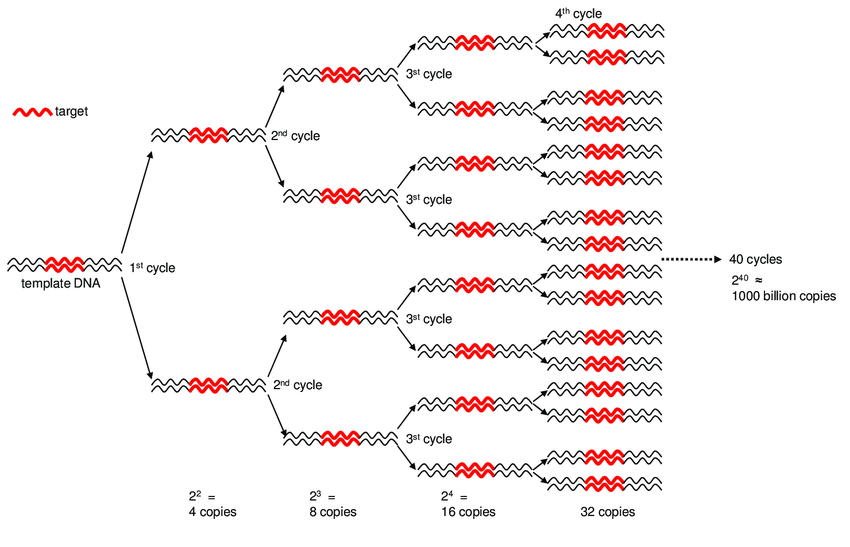
\includegraphics[scale=0.5]{Chapter2Images/amp.png}
\caption{Assuming that the qPCR runs with perfect efficiency, we expect to see a doubling of DNA after every cycle \citep{foodscience}.}
\label{fig:amp}
\end{figure} 

\newpage



Figure~\ref{fig:amp} is a basic visualization of how qPCR works. At each cycle, assuming perfect efficiency, the amount of target DNA should double.

\vspace{5mm}

To measure concentration of DNA, a fluorometer detects levels of fluorescence as the thermal cycler runs, and the level of fluorescent signal reflects the amount of target DNA in the sample. During the first cycles, the amount of fluorescence produced is not significant enough to separate from background light. As the experiment progresses, the fluorescent signal may increase above a certain detectable level (corresponding to the initial number of template DNA). This point is known as the `Quantification Cycle' or the Cycle Threshold (CT). This value allows for the detection and quantification of target DNA \citep{ctmethod}. Typically, a specified number of cycles is decided on as a `cutoff' value. That is, if we have gone through a specified number of cycles, and still have not detected a signal, we would consider this to be indicative that the target DNA was not present in the sample.



\vspace{5mm}


In other words, as the experiment progresses, fluorescence is observed when the specified target DNA is detected. If it only takes a few cycles, this results in a low Cycle Threshold (`CT') score and indicates high levels of target DNA were present in the sample. The more cycles it takes to detect a visible fluorescence signal, the higher the CT score, indicating that less of the target DNA is present in the sample \citep{dropletqpcr,independentreplicates}.

\vspace{5mm}

Another concept that is often used when discussing eDNA related studies is the `Limit of Detection' or `LoD'. With respect to eDNA studies, the `LoD' is defined as the minimum amount of target DNA required to conclude with high probability that specified target DNA exists in the sample. Researchers often agree upon a CT value to determine a LoD. For example, in our later research we define the LoD to be CT $<$ 50. Hence, if there is still no visible fluorescence after 50 cycles (i.e. CT $>$50), we conclude that the sample does not contain the target DNA. In other cases, LoD may be defined in terms of the number of copies of target DNA.

\newpage

\section{Biomass and eDNA concentration}

The study by \cite{biomass} deals directly with estimation of fish biomass from eDNA concentration and helps to illustrate how statistical analysis is performed on eDNA data.

\vspace{5mm}

In this study, researchers hypothesized that eDNA released from the common carp, \textit{Cyprinus carpio} is positively correlated with the carp's biomass. Furthermore, researchers extended their knowledge of eDNA to study carp in the field, where they incorporated several environmental covariates into their statistical models.

\vspace{5mm}

To study collected samples of carp eDNA, researchers used a carp specific mitochondrial gene fragment. To construct the standard curve, qPCR was conducted on the target species using a pGEM-T Easy Vector, and a dilution series of the carp DNA containing 30 to 30,000 copies of DNA was created. This involved plotting the absorbance obtained using known concentrations of carp DNA. Using the standard curve for carp, researchers were able to obtain estimates for the number of copies of carp DNA in each sample they ran. Water that was collected as samples was immediately filtered using a centrifuge. 

\vspace{5mm}

Since one copy of carp DNA was detected in each triplicate, the Limit of Detection (LoD) for carp DNA was chosen to be a detection of at least one copy of carp specific DNA. Three technical replicates (sub samples from the same triplicate) were run on each sample and if a technical replicate showed a negative result, it was assigned a value of zero. The mean value obtained in the three replicates was the quantity chosen to be used in regression. In addition, three wells containing no carp DNA were used as negative controls. In each of the three wells chosen to be negative controls, no eDNA of carp was detected.

\vspace{5mm}

The first experiment was done using tanks. Juvenile carp in the Mie Prefecture of Japan were captured and transferred to a lab in Kyoto.
To study the impact of biomass, twelve tanks were used.  Four tanks had only one carp, four tanks had five carps and the other four tanks contained ten carps. The water temperature was kept constant among the separate tanks. On the sixth day, triplicate samples of 50mL were collected from each tank. 


\begin{figure}[H]
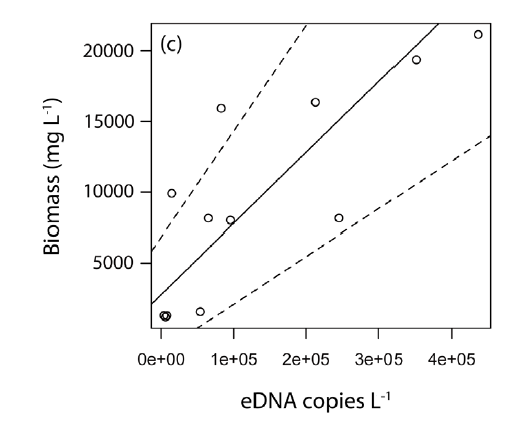
\includegraphics{Chapter2Images/eDNAcopies.png} 
\caption{This figure is a plot of data obtained of biomass concentration (y-axis) versus eDNA copies per Litre (x-axis). There was a
significant positive correlation between the number of eDNA
copies and carp biomass per 1 L (y = 0.050x+2789, $R^{2}$ =0.66,
p= 0.001). There are twelve points, one for each tank used in the tank experiment. There is an overlapping of three points in the bottom left hand side of the figure
 \citep{biomass}.}
\label{fig:copies}
\end{figure}


  Figure~\ref{fig:copies} shows the result of linear regression applied to the qPCR data. Using linear regression, researchers were able to obtain estimates of coefficients and estimates of standard errors. In this experiment, linear regression was able to provide an adequate analysis with moderate explanatory power. The $R^{2}=0.66$ indicates that this linear model does a moderate job in explaining the variance in the data. The dashed lines show the associated confidence bands for the regression estimate. We also show later in our analysis that linear regression can be used as a reliable method for obtaining estimates of Coho biomass. 


\vspace{5mm}

To bridge the research into the field, researchers collected water samples from Lake Biwa in Japan. The area of the lake in which they sampled was known to be inhabited by the common carp. From 21 distinct sites on the lake, 2-L samples of water were collected. Moreover, several environmental covariates were recorded such as water temperature, conductivity, etc. The samples were immediately transferred  back to the lab where they were extracted and analyzed using the same standard curve for carp. All sequences from which the eDNA analysis indicated presence of carp, were confirmed to be regions of the lake that did contain carp.


\vspace{5mm}

 In this experiment, researchers made use of General Linear Models and Stepwise selection. By comparing $R^{2}$ values, researchers were able to make conclusions regarding which covariates should be included in models. The model that included water temperature as a covariate turned out to work best in the field experiment and several environmental covariates such as pH or chlorophyll were seen to not be significant.


\begin{figure}[H]
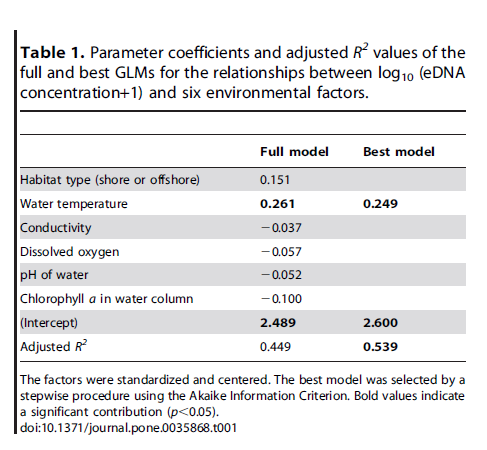
\includegraphics{Chapter2Images/biomassGLM.png} 
\caption{ Table summarizing the various estimates and adjusted $R^{2}$ values for a full model and the best model.
 \citep{biomass}.}
\label{fig:glm}
\end{figure}

\newpage

 Figure~\ref{fig:glm} summarizes the result of the general linear model that researchers created to evaluate the relationship between eDNA concentration and several environmental covariates. The full model contains all the above environmental covariates and has an adjusted $R^{2}$=0.449. On the other hand, the best model only contains an intercept and water temperature, and the adjusted $R^{2}$ is improved to 0.539.

\vspace{5mm}

Prior to fitting a general linear model, researchers used a variance inflation factor (VIF) to assess whether there was collinearity among the covariates. This was done by dividing the variance estimates of the full model by the variance estimates of a model that only included one term at a time. Calculating the VIF for each covariate indicated that there was not sufficient evidence to conclude that collinearity existed among any of the covariates (this was done by ensuring that the VIF was not too large, in particular, less than a common cutoff value of 5 for all covariates). The eDNA estimates were obtained as above using qPCR and comparison to the standard curve, and a log10 transformation was applied to the estimates in an effort to normalize the results. A Shapiro Wilks test applied to the residuals confirmed normality of the estimates at a 95 percent confidence level.  To select the best GLM, researchers compared models using stepwise selection based on AIC criteria. In this case, the best general linear model included the temperature of the water as an environmental covariate. Moreover, the estimate for water temperature was  significantly positive.

\vspace{5mm}

In Chapter 5, we also use a stepwise selection approach to determine which environmental covariates to include in our field models.



\section{eDNA and Species Occupancy}
 
The study by \cite{parasite} further helps to illustrate the methods in which eDNA can be used to make inference regarding target organism occupancy. The \textit{Schistocephalus solidus}-threespine stickleback pair is a commonly researched parasite/host pair. \textit{Schistocephalus solidus} is a parasitic flatworm, while the abdominal cavity of the  \textit{Gasterosteus aculeatus} (threespine stickleback) is one possible host location for this parasite. Conventional  methods for detecting if a stickleback is infected with the parasite is by simple visual detection. However, this results in not identifying parasites that are too small or have not yet grown to full size (past a certain mass threshold). 


\vspace{5mm}

An alternative, non-invasive method to detect the parasitic tapeworm involves using qPCR to test for the presence of \textit{Schistocephalus solidus} eDNA. Researchers took samples from the abdominal cavity of sticklebacks and performed qPCR to test for \textit{Schistocephalus solidus} DNA. Using this method, scientists were able to correctly assign the status to 98 percent of n=151 fish.
Moreover, not only did qPCR allow for the detection, but it also allowed for a comparative quantification of eDNA. That is, researchers were able to get an idea of how large the parasite was simply based on the results of the qPCR. Lower CT scores indicated higher presence of eDNA and was correlated with larger parasite mass. 

\vspace{6mm}

Researchers used minnow traps in Lac Temiscouata and Isle-Vertes (Quebec, Canada) to capture the sticklebacks. The fish were transferred to Laval University where they were maintained according to their natural requirements. In total, 96 fish were sampled from Lac Temiscoutata and 55 were sampled from Isle-Vertes. By the time the experiment began, all fish were considered to be adult fish. The fish were each subsequently isolated into 2 L tanks in the lab.

\vspace{5mm}

The fish were removed individually and placed on sponges. A small 1ml volume syringe filled with 100 $\mu L$ of a phosphate buffer was injected into the abdominal cavity of the fish. Without removing the needle, the syringe was pulled back until it had 100  $\mu L$ of the recently injected buffer back in the needle. The needle was then removed, and the fish was returned to its tank. This removed liquid was added directly to a tube containing 700 $\mu L$ of  Longmire Lysis preservation buffer. This was done once per day for each fish on two consecutive days. The samples were then stored in an appropriate environment to maintain the delicate structure of the DNA. Note that on the second sample, the phosphate buffer was added to the same tube containing the 700$ \mu L$ of lysis buffer from the previous day. Hence, each tube had up to 900 $\mu L$ of liquid.
Once the fish had been sampled twice, they were killed with an injection of MS-222 and dissected. Fish size, sex and mass were recorded as well as the mass and number of any  \textit{Schistocephalus solidus} parasites in the fish. A `PI' value was calculated where PI= [total mass of parasite (mg) / total mass of host plus parasite (mg)]x100.


\vspace{5mm}

To detect DNA from the parasite, researchers used a pair of primers that amplified a specific sequence from a nuclear gene in the \textit{Schistocephalus solidus} genome. The specific gene sequence has no known analogs in other species. PCR assays were then tested on genomic DNA to confirm that the primers indeed amplified the parasite DNA and did not falsely amplify other DNA from the stickleback.

\vspace{6mm}

Prior to the experiment, researchers obtained what is known as a `Standard Curve' for \textit{S.solidus} genomic DNA. A `Standard Curve', also known as a `Calibration Curve' allows researchers to make inference about DNA concentrations using previous knowledge of that species DNA \citep{standardCurve}. In this case, researchers used known concentrations of \textit{S. solidus} DNA obtained from three individuals and prepared a wide range of dilutions. At the low end, researchers prepared a 0.01 ng $\mu L^{-1}$ sample and at the high end a 0.9 ng$ \mu L^{-1}$ sample. Researchers also created multiple samples with known concentrations in between the minimum and maximum values. These solutions are referred to as the `standard solutions'.  The fluorescence produced by cycling these standard solutions was then measured using a spectrophotometer and the results were recorded. A graph was produced showing the relation between concentration of eDNA and the CT value. This is known as a `Standard Curve'.  Hence, the Standard curve allowed researchers to make conclusions about new DNA concentrations using prior knowledge of the properties of that specific target DNA. 

\vspace{5mm}

Finally, researchers were able to begin to analyze the eDNA. The removed eDNA was amplified using qPCR and the primers described. CT values were recorded when the fluorescence reached a certain threshold. Researchers included negative controls (no DNA and no primers) in each plate. Each reaction was done in triplicate. 

\vspace{5mm}

 Once the qPCR amplification had taken place, the presence or absence of eDNA in the fish was determined by comparing the obtained CT values with the standard curve. If more than 70 cycles of qPCR were needed, this was considered to be `undetermined' for the presence of parasite eDNA.

\vspace{5mm}
 For each fish, if at least one of the three CT values was less than 70, this was considered a positive identification of the parasite. If the CT was undetermined for all three replicates (more than 70 cycles) it was also considered a negative. The CT value used for analysis was the lowest CT value obtained among the three replicates. Hence, if the CT was only undetermined for one sample, then the lowest CT score among the other two replicates was used. If it was undetermined for two replicates, then the CT of the remaining replicate was used.

\vspace{5mm}

Statistical analysis was done using the R programming language \citep{Rprogram}. Researchers used a non-parametric Spearman correlation to test whether the eDNA concentration (estimates obtained by comparing CT values collected during qPCR to the previously defined standard curve) negatively correlated with the parasite mass. The results of the experiment were promising. In total, of the 151 fish collected, 35 were infected with parasites. Using eDNA, researchers correctly predicted 32 of the 35 infected fish. Hence only 3 infected fish were incorrectly classified. Of the 116 fish that had no parasites, researchers never falsely predicted infection. A CT value of less than 70 was used as the detection cutoff.

\vspace{5mm}

We define True Positive (TP) to be the number of infected fish that were classified as infected, True Negative (TN) as the number of non-infected fish that were classified as non-infected, False Positive (FP) to be the number of fish incorrectly classified as infected and False Negative (FN) as the number of fish incorrectly classified as having no parasite. In this example, TP=32,
TN=116, FP=0 and FN=3. Using these definitions, we calculated some key statistical values such as accuracy, sensitivity and specificity \citep{statisticallearning}. 

\vspace{5mm}

Firstly, we calculated accuracy= $\frac{TP+TN}{TP+TN+FP+FN}=\frac{32+116}{32+116+3}=0.9801$

Secondly, we calculated sensitivity=$\frac{TP}{TP+FN}=\frac{35}{35+3}=0.914$

and we calculated the specificity=$\frac{TN}{TN+FP}=\frac{116}{116+0}=1$

\vspace{5mm}

Hence, we see that the researchers were very accurate. The testing also had perfect specificity, which means that researchers never predicted that a healthy fish had a parasite.



\newpage

A scatterplot of parasite mass versus CT confirms what we would expect. High parasitic mass is associated with lower CT values. This is supported by the negative Spearman correlation of -0.41; although, the variance appears to be somewhat high despite a clear trend. In this experiment, the study of eDNA alone produced highly accurate identification of infected versus non-infected species. Figure~\ref{fig:parasite} shows the lowest CT value obtained from the three replicates for each of the organisms that were confirmed visually to have a parasite \citep{parasite}.



\begin{figure}[H]
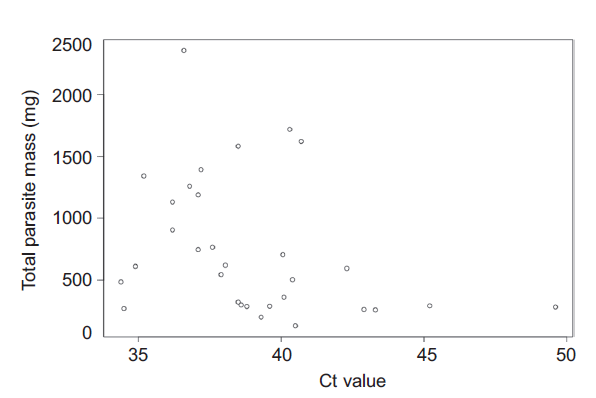
\includegraphics{Chapter2Images/parasitect.png} 
\caption{eDNA concentration co-varies with total parasite mass. ` Low cycle threshold (CT) values, which represent high levels of eDNA, are associated with a high parasite mass (Spearman correlation=-0.41, P=0.01, n=31) '.  The CT value plotted is the lowest value obtained from among the three replicates \citep{parasite}.}
\label{fig:parasite}
\end{figure}

Figure~\ref{fig:parasite} is a visualization of the CT scores obtained for the diseased fish. In general, parasite mass was negatively correlated with CT score. One fish was removed from the original 32 as it died before dissection could be performed. Hence there are 31 points plotted.

